\documentclass[a4paper,11pt]{article}
\usepackage[utf8]{inputenc}
\usepackage{amsmath}
\usepackage{amsfonts}
\usepackage{amssymb}
\usepackage{graphicx}
\usepackage{braket}

\numberwithin{equation}{section}
%\renewcommand\thesubsection{\alph{subsection}}
\newcommand{\bvp}[1]{\mathbf{#1}'}
\newcommand{\bv}[1]{\mathbf{#1}}
\newcommand{\ez}{\epsilon_0}
\newcommand{\eo}{\epsilon_1}
\newcommand{\lrp}[1]{\left({#1}\right)}
\newcommand{\lrb}[1]{\left\{{#1}\right\}}


%opening
\title{Electromagnetic Theory II HW5}
\author{Vince Baker}

\begin{document}

\maketitle

\section{7.19}
For each wavefunction we will evaluate the Fourier transform of $u(x,0)$ to determine $A(k)$.
The normalized RMS deviation is defined by:
\begin{align}
 \Delta f = \lrp{\frac{\int \lrp{(x-\bar{x})f(x)}^2 dx}{\int (f(x))^2 dx}}^{1/2}
\end{align}
a) We take the Fourier transform of $u(x,0) = Ne^{-a|x|/2}e^{ik_0x}$:
\begin{align}
 A(k) &= \frac{1}{\sqrt{2\pi}}\int_{-\infty}^\infty Ne^{-a|x|/2}e^{ik_0x}e^{-ikx}dx\\
 A(k) &= \frac{N}{\sqrt{2\pi}}\int_{-\infty}^\infty e^{-i(k-k_0)x}e^{-a|x|/2} dx\\
 A(k) &= \frac{2N}{\sqrt{2\pi}}\int_{0}^\infty \lrp{\cos{((k-k_0)x)}-i\sin{((k-k_0)x)}} e^{-a|x|/2} dx
\end{align}
For any reasonably localized wave packet the integral will be zero outside of a finite region of support.
The wave packets considered in this problem are all symmetric: therefore, the odd sine term in the integral will be zero.
\begin{align}
 A(k) &= \frac{2N}{\sqrt{2\pi}}\int_{0}^\infty \cos{((k-k_0)x)} e^{-a|x|/2} dx\\
 A(k) &= \frac{2N}{\sqrt{2\pi}}\lrp{\frac{2a}{a^2+4(k-k_0)^2}}\\
 A(k) &= \frac{N}{\sqrt{2\pi}}\lrp{\frac{a}{a^2/4+(k-k_0)^2}}\\
 |A(k)|^2 &= \frac{N^2}{2\pi}\lrp{\frac{a}{a^2/4+(k-k_0)^2}}^2
\end{align}
Where we have assumed $a>0$ (since otherwise the interval will not converge).
We take $a=1, k_0=0, N=1$ and plot the wave packet and the spectrum (figure 1).
\\ \\
Using eq. 1 we can calculate the RMS deviations.
We note that $\bar{x}=0$, and we can also set $k_0=0$ for convenience.
\begin{align}
 \Delta_x &= \sqrt{\frac{2/a^3}{1/a}} = \frac{\sqrt{2}}{a}\\
 \Delta_k &= \sqrt{\frac{\pi/a}{4\pi/a^3}} = \frac{a}{2}\\
 \Delta_x \times \Delta_k &= \frac{\sqrt{2}}{2} > \frac{1}{2}
\end{align}
\\
b) We take the Fourier transform of $u(x,0) = Ne^{-a^2|x|^2/4}e^{ik_0x}$:
\begin{align}
 A(k) &= \frac{1}{\sqrt{2\pi}}\int_{-\infty}^\infty Ne^{-a^2|x|^2/4}e^{ik_0x}e^{-ikx}dx\\
 A(k) &= \frac{2N}{\sqrt{2\pi}}\int_{0}^\infty \cos{(k-k_0)x} e^{-a^2|x|^2/4} dx\\
 A(k) &= \frac{N}{\sqrt{2\pi}}\lrp{\sqrt{4\pi/a^2}e^{-(k-k_0)^2/a^2}}\\
 A(k) &= \frac{\sqrt{2}N}{a}e^{-(k-k_0)^2/a^2}\\
 |A(k)|^2 &= \frac{2N^2}{a^2}e^{-2(k-k_0)^2/a^2}
\end{align}
We take $a=1, k_0=0, N=1$ and plot the wave packet and the spectrum (figure 2).

Using eq. 1 we can calculate the RMS deviations.
We note that $\bar{x}=0$, and we can also set $k_0=0$ for convenience.
\begin{align}
 \Delta_x &= \sqrt{\frac{\sqrt{2\pi}/a^3}{2\sqrt{2\pi}/a}} = \frac{1}{a}\\
 \Delta_k &= \sqrt{\frac{\sqrt{\pi/2}a^3/4}{\sqrt{\pi/2}a}} = \frac{a}{2}\\
 \Delta_x \times \Delta_k &= \frac{1}{2}
\end{align}
So a Gaussian wave packet minmizes the joint uncertainty in localization and frequency.
\\
c) We take the Fourier transform of $u(x,0) = N(1-a|x|)e^{ik_0x}\ (a|x|<1)$:
\begin{align}
 A(k) &= \frac{1}{\sqrt{2\pi}}\int_{-1/a}^{1/a} N(1-a|x|)e^{ik_0x}e^{-ikx}dx\\
 A(k) &= \frac{2N}{\sqrt{2\pi}}\int_{0}^{1/a} \cos{((k-k_0)x)} (1-ax) dx\\
 A(k) &= \frac{2N}{\sqrt{2\pi}}\lrp{\frac{a-a\cos{((k-k_0)/a)}}{(k-k_0)^2}}\\
 |A(k)|^2 &= \frac{N^2}{2\pi}\lrp{\frac{a-a\cos{((k-k_0)/a)}}{(k-k_0)^2}}^2
\end{align}
We take $a=1, k_0=0, N=1$ and plot the wave packet and the spectrum (figure 3).

Using eq. 1 we can calculate the RMS deviations.
We note that $\bar{x}=0$, and we can also set $k_0=0$ for convenience.
The first integral can be done with the substitution $x' = x/a$:
\begin{align}
 \Delta_x &= \frac{1}{a} \sqrt{\frac{1/15}{2/3}}= \frac{1}{\sqrt{10}a}\\
 \Delta_k &= \sqrt{\frac{\pi a}{\pi/3a}} = \sqrt{3}a\\
 \Delta_x \times \Delta_k &= \sqrt{3/10} > \frac{1}{2}
\end{align}
\\
d) We take the Fourier transform of $u(x,0) = Ne^{ik_0x}\ (|x|<a)$:
\begin{align}
 A(k) &= \frac{1}{\sqrt{2\pi}}\int_{-a}^{a} Ne^{ik_0x}e^{-ikx}dx\\
 A(k) &= \frac{2N}{\sqrt{2\pi}}\int_{0}^{a} \cos{((k-k_0)x)} dx\\
 A(k) &= \frac{2N}{\sqrt{2\pi}}\lrp{\frac{\sin{a(k-k_0)}}{k-k_0}}\\
 |A(k)|^2 &= \frac{2N^2}{\pi}\frac{\sin^2{(a(k-k_0))}}{(k-k_0)^2}
\end{align}
We take $a=1, k_0=0, N=1$ and plot the wave packet and the spectrum (figure 4).

Using eq. 1 we can calculate the RMS deviations.
We note that $\bar{x}=0$, and we can also set $k_0=0$ for convenience.
\begin{align}
 \Delta_x &= \sqrt{\frac{2a^3/3}{2a}}= \frac{a}{\sqrt{3}}\\
 \Delta_k &= \sqrt{\frac{\infty}{a\pi}} = \infty\\
 \Delta_x \times \Delta_k &= \infty > \frac{1}{2}
\end{align}

\begin{figure}[p]
 \caption{Part A}
 \centering
   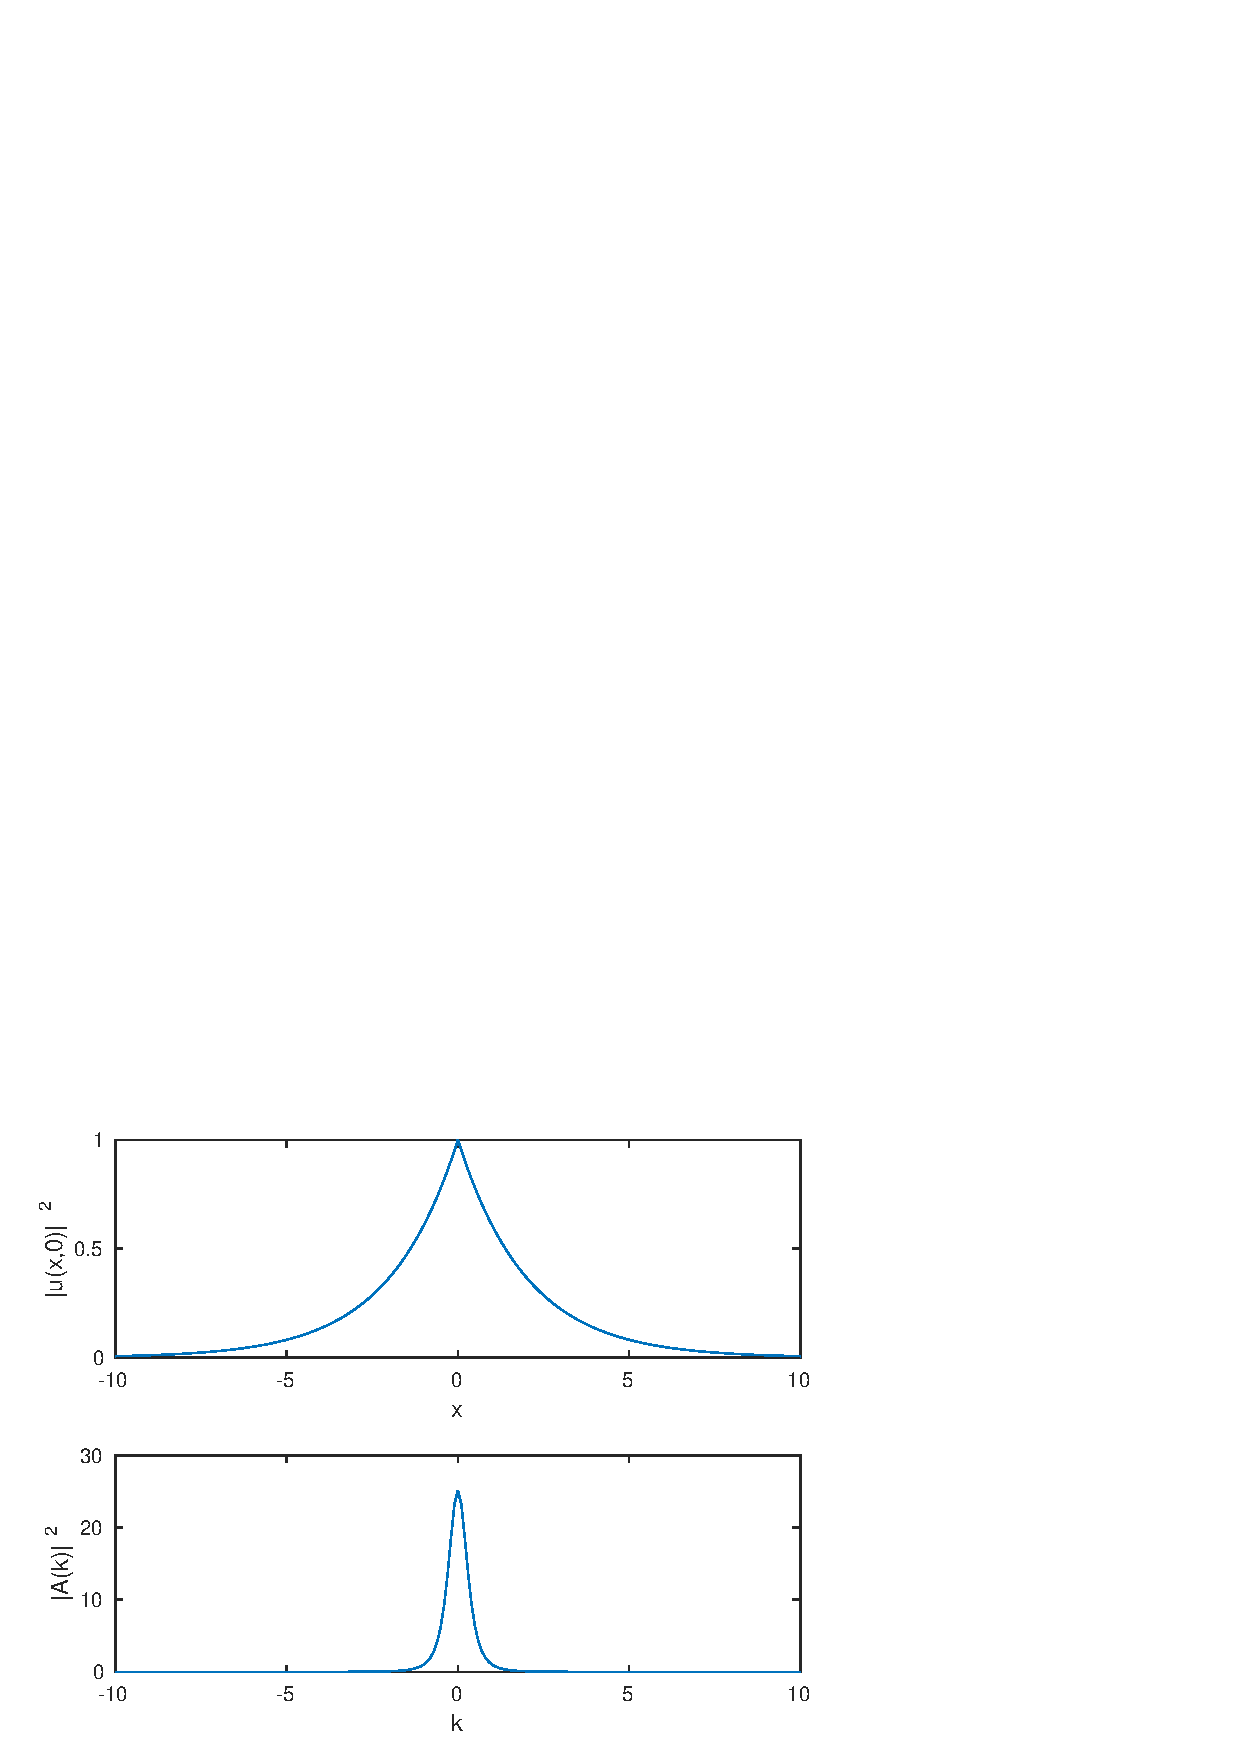
\includegraphics[width=\textwidth]{a}
\end{figure}

\begin{figure}[p]
 \caption{Part B}
 \centering
   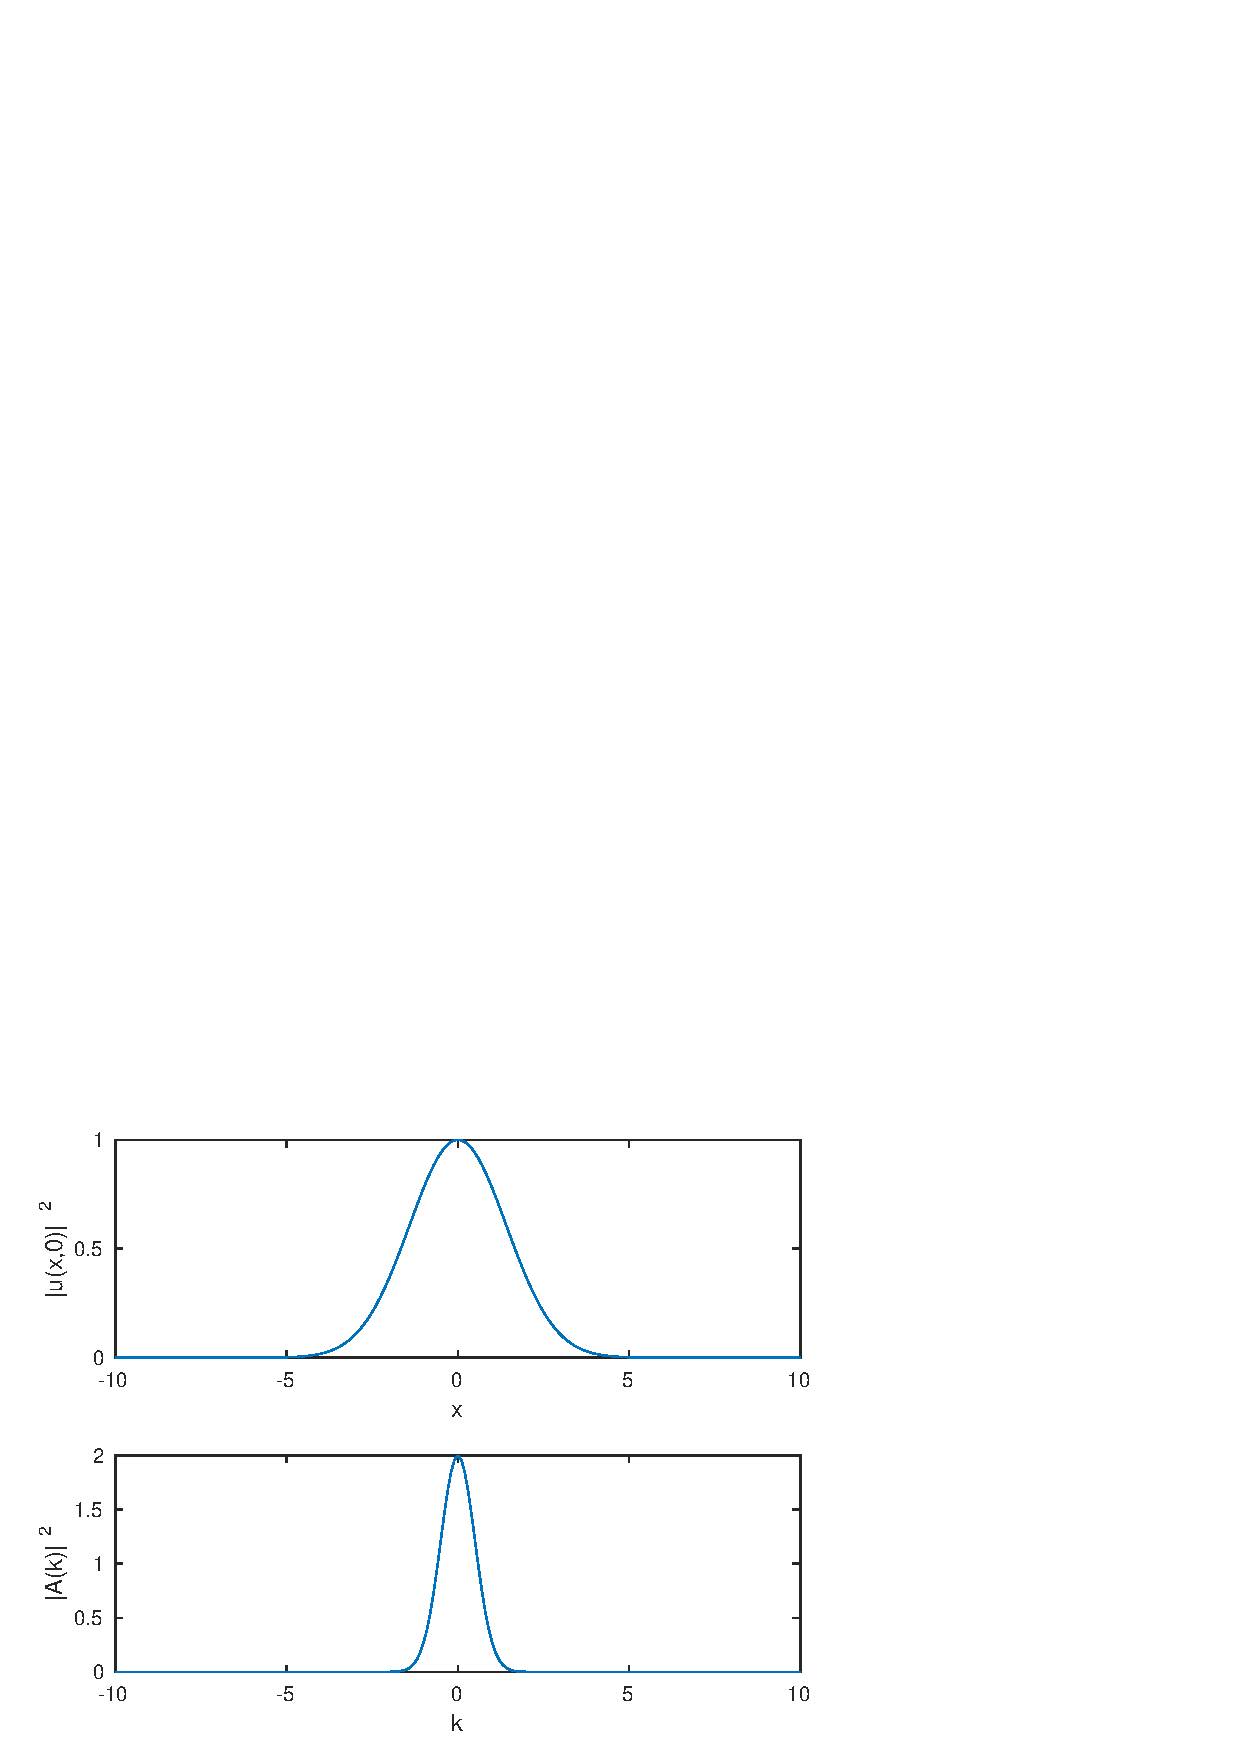
\includegraphics[width=\textwidth]{b}
\end{figure}

\begin{figure}[p]
 \caption{Part C}
 \centering
   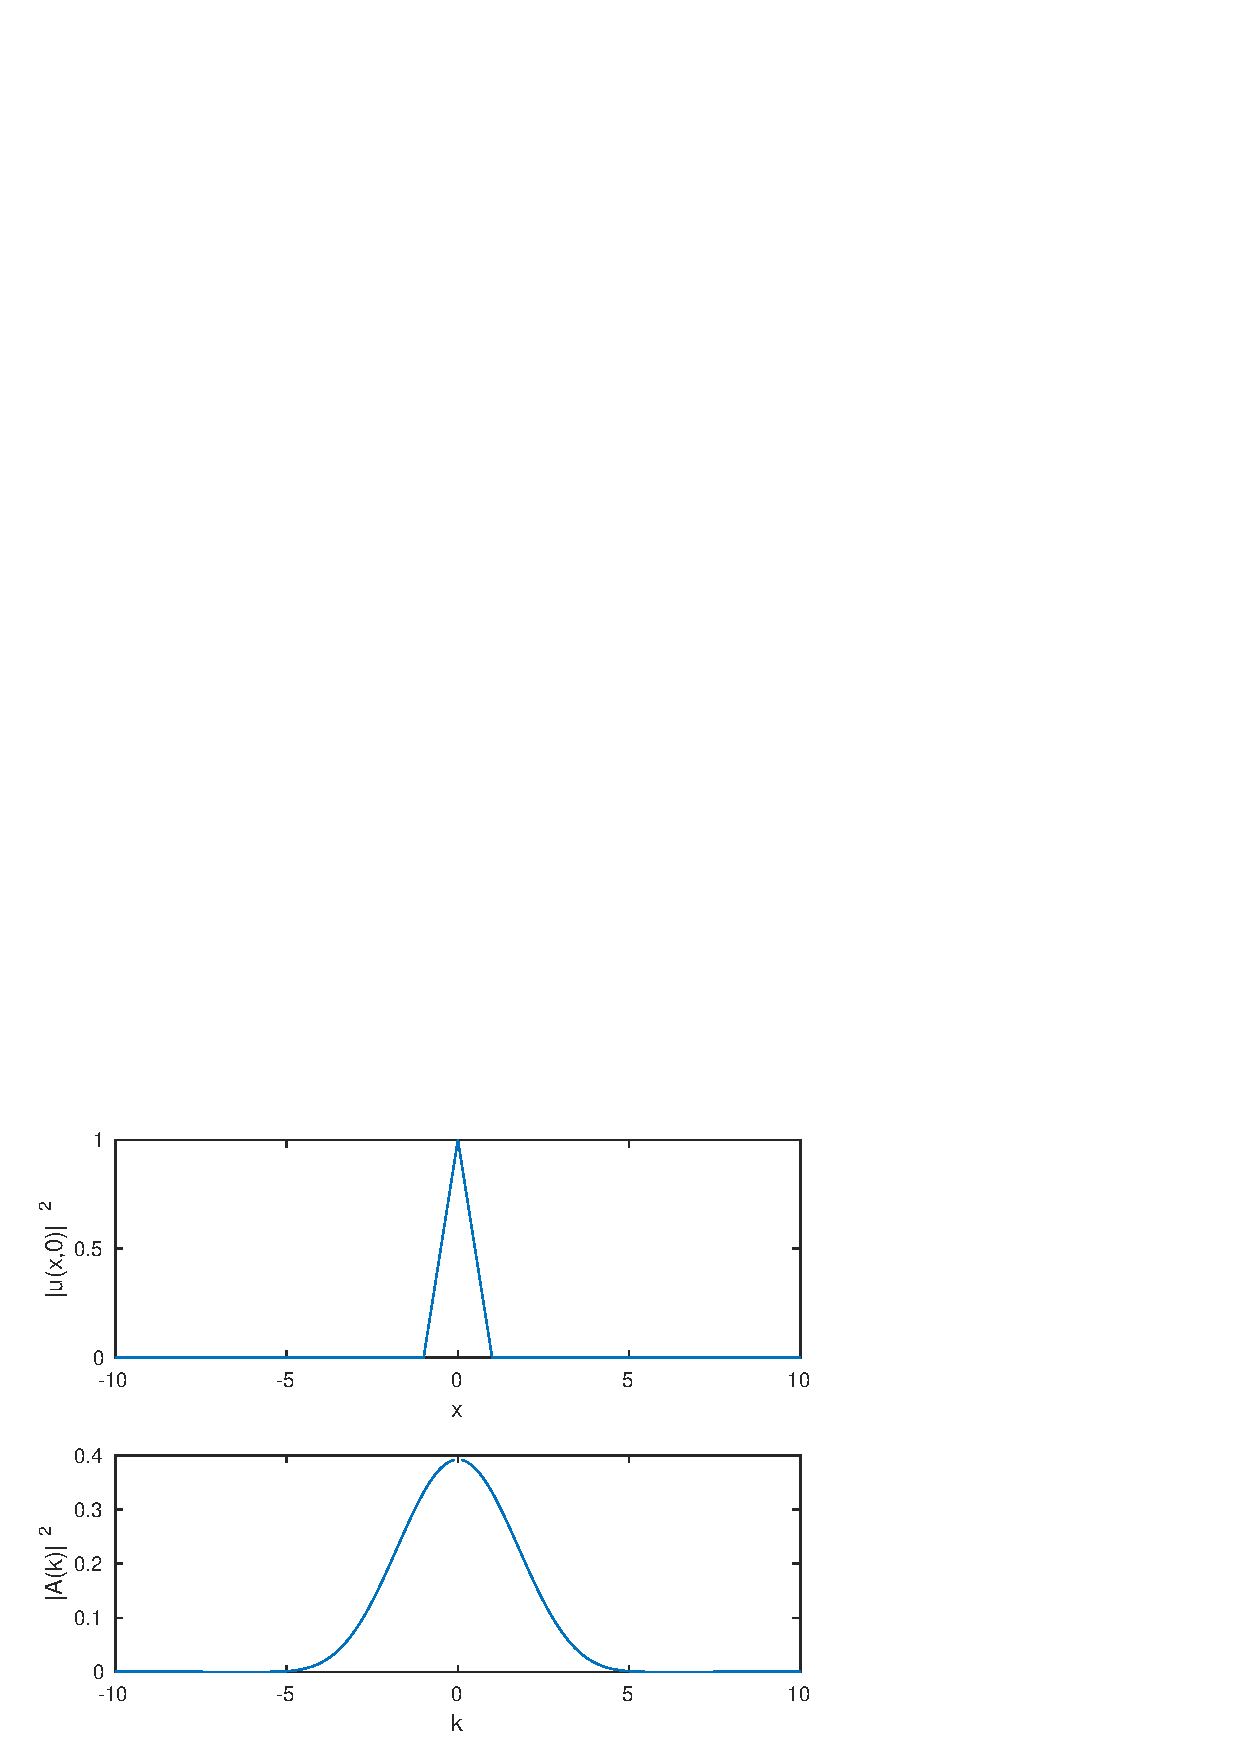
\includegraphics[width=\textwidth]{c}
\end{figure}

\begin{figure}[p]
 \caption{Part D}
 \centering
   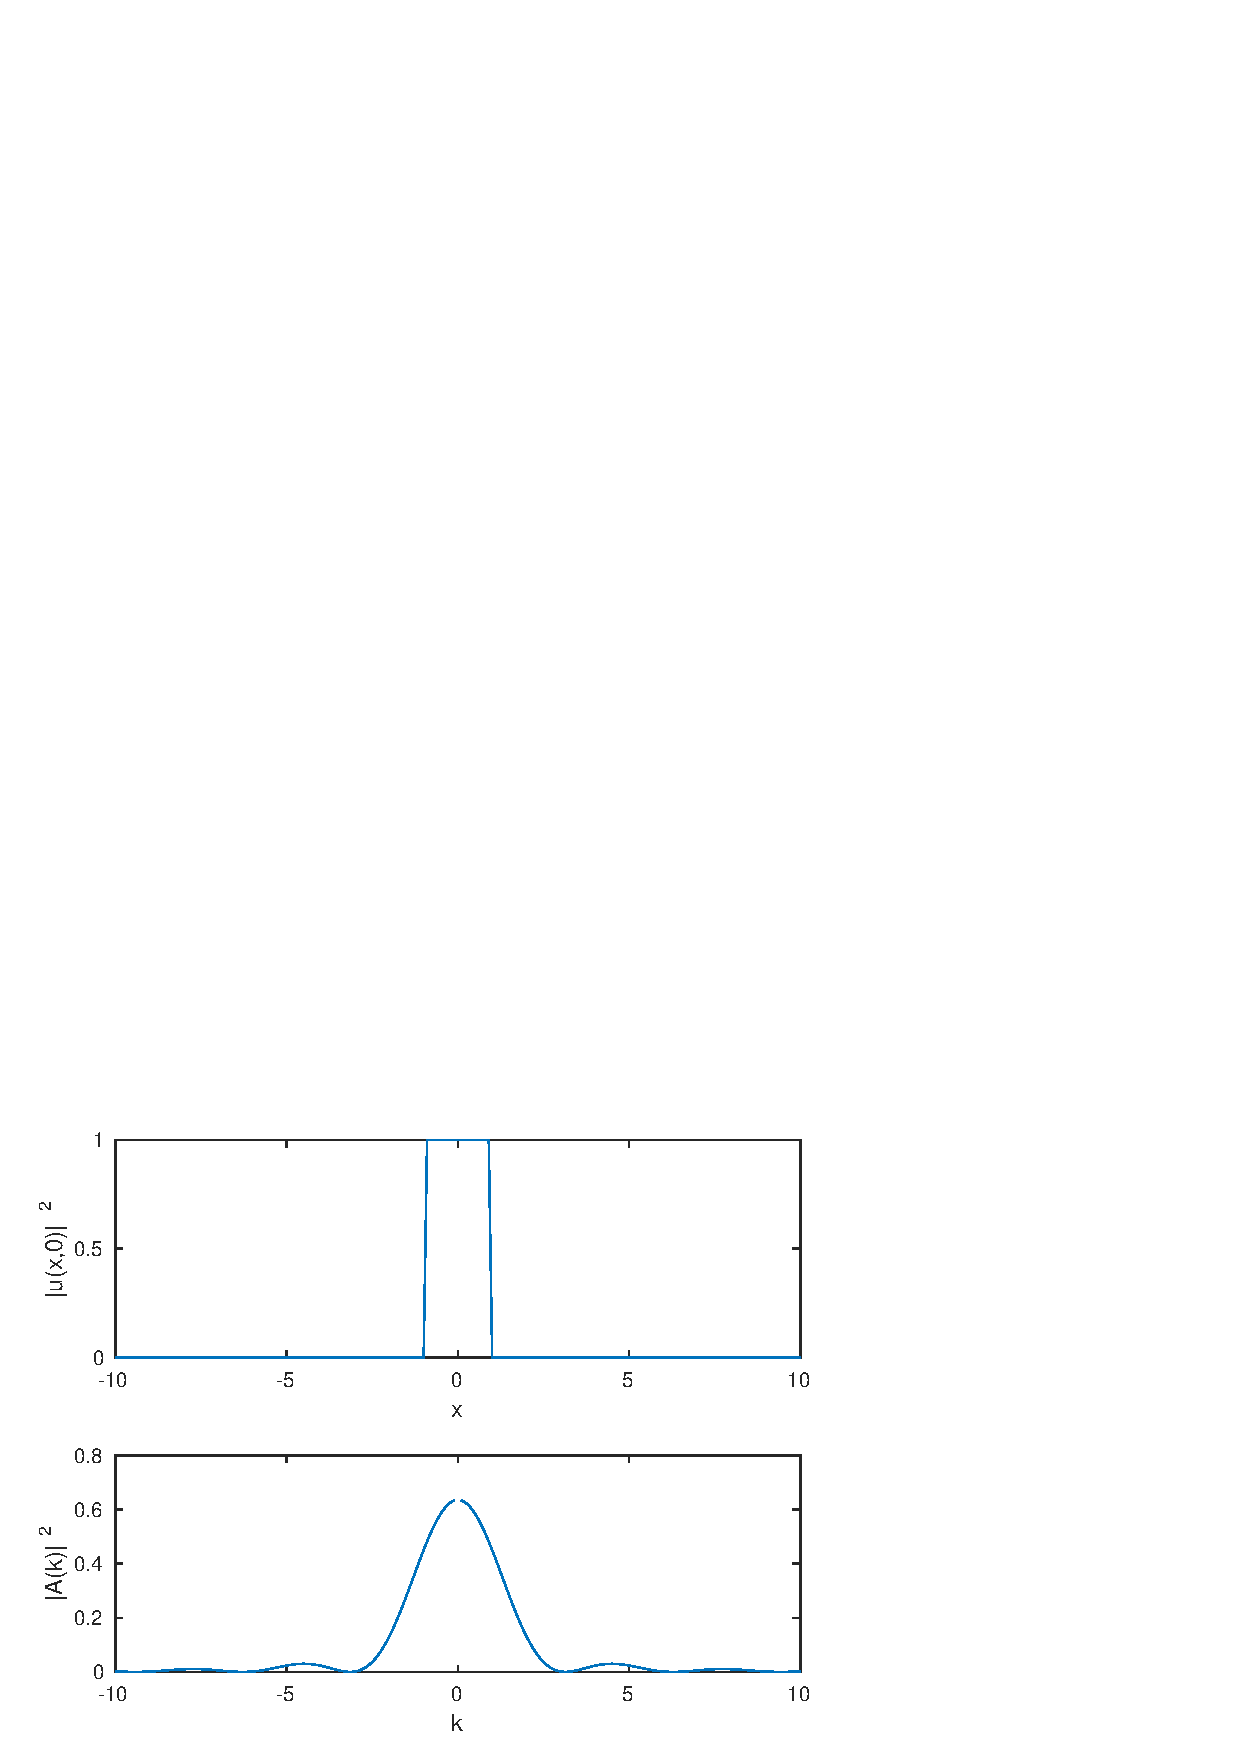
\includegraphics[width=\textwidth]{d}
\end{figure}

\section{8.2abc}
a) For a TEM mode both the electric and magnetic fields are perpendicular to the direction of propagation.
We first solve the static problem defined by:
\begin{align}
 \nabla_t \times \bv{E} &= 0\\
 \nabla_t \cdot \bv{E} &= 0\\
 \bv{B} = \pm \sqrt{\mu\epsilon}\hat{\bv{z}} \times \bv{E}
\end{align}
The electric field at the surface of the conductors has only a normal component.
From (1) the electric field points in the radial direction, and from (2):
\begin{align}
 \frac{1}{\rho}\frac{\partial}{\partial \rho}\lrp{\rho E} &= 0\\
 E &= -\rho\frac{\partial E}{\partial \rho}\\
 E &= C\frac{1}{\rho}\\
 B &= C\sqrt{\mu\epsilon}\frac{1}{\rho}\hat{\phi}\\
 H &= C\sqrt{\frac{\epsilon}{\mu}}\frac{1}{\rho}\hat{\phi}
\end{align}
At $\rho=a$ we set $H=H_0,\ C=H_0\sqrt{\frac{\mu}{\epsilon}}a$ leading to the solutions:
\begin{align}
 \bv{E} &= H_0\sqrt{\frac{\mu}{\epsilon}}\frac{a}{\rho}\hat{\rho}\\
 \bv{H} &= H_0\frac{a}{\rho}\hat{\phi}
\end{align}
The time-averaged power flow per unit area is $\frac{1}{2}Re(\bv{E}\times \bv{H}^*)$:
\begin{align}
 <\bv{S}> &= \frac{1}{2}H_0^2\sqrt{\frac{\mu}{\epsilon}}\frac{a^2}{\rho^2}\hat{z}
\end{align}
We now integrate the flux across the cross-sectional area of the waveguide to find the total power flow:
\begin{align}
 P &= \int_a^b \int_0^{2\pi} <\bv{S}>\rho\ d\rho\  d\phi\\
 P &= H_0^2\sqrt{\frac{\mu}{\epsilon}}\pi a^2 \int_a^b \frac{1}{\rho}\ d\rho\\
 P &= H_0^2\sqrt{\frac{\mu}{\epsilon}}\pi a^2\ln{(b/a)}
\end{align}
\\
b) For a reasonably good conductor the power loss is of the form (Jackson 8.56 and 8.57):
\begin{align}
 P(z) &= P_0e^{-2\beta_\gamma z}\\
 \beta_\gamma &= -\frac{1}{2P}\frac{dP}{dz}
\end{align}
The power lost into a unit area of the non-ideal conductor is:
\begin{align}
 \frac{dP_{loss}}{da} &= \frac{1}{2\sigma\delta}|K_{eff}|^2\\
 \frac{dP_{loss}}{da} &= \frac{1}{2\sigma\delta}H_0^2\frac{a^2}{\rho^2}
\end{align}
The total power lost per unit length will include contributions from both the inner and outer conductor.
Integrating over both surfaces:
\begin{align}
 \frac{dP}{dz} &= \frac{\pi}{\sigma\delta}H_0^2a^2\lrp{\frac{1}{a}+\frac{1}{b}}
\end{align}
We can now calculate the loss per unit length:
\begin{align}
 \beta_\gamma &= -\frac{1}{2\sigma\delta}\sqrt{\frac{\epsilon}{\mu}}\frac{\lrp{1/a+1/b}}{\ln{(b/a)}}
\end{align}
We have thus proved the desired form for power attenuation along the waveguide.
\\
c) The characteristic impedance can be found from the voltage difference between the conductors and the current flowing along either conductor.
To find the potential difference we integrate the E field (9) along a radial from a to b:
\begin{align}
 V &= \int_a^b H_0\sqrt{\frac{\mu}{\epsilon}}\frac{a}{\rho}\ d\rho\\
 V &= H_0\sqrt{\frac{\mu}{\epsilon}}a\int_a^b \frac{1}{\rho}\ d\rho\\
 V &= H_0\sqrt{\frac{\mu}{\epsilon}}a\ln{(b/a)}
\end{align}
For the current along a conductor we can use the approximate effective current from (18) $K_{eff} = H_0\frac{a}{\rho}$.
For the inner conductor the effective current is just $H_0$, so the total current flowing along the inner cylinder is $2\pi a H_0$.
The ratio of the voltage to the current gives the characteristic impedance:
\begin{align}
 Z_0 &= \frac{1}{2\pi}\sqrt{\frac{\mu}{\epsilon}}\ln{(b/a)}
\end{align}







\end{document}
